\section{Error mitigation for VQE} \label{sec:error-mit}

When the noise of a quantum computer is below a certain threshold and a sufficient number of qubits are available, quantum error correction schemes can be applied to suppress the noise to arbitrarily small levels~\cite{nielsenQuantumComputationQuantum2010}. However, hardware demonstrations of simple quantum error correcting codes have been limited and have only demonstrated fault-tolerant universal quantum computation with limited error-correcting capabilities
%none have demonstrated a functional fault-tolerant platform for universal quantum computation yet
\cite{andersenRepeatedQuantumError2020a,barendsSuperconductingQuantumCircuits2014,campagne-ibarcqQuantumErrorCorrection2020,niggQuantumComputationsTopologically2014,ofekExtendingLifetimeQuantum2016,waldherrQuantumErrorCorrection2014,Postler_2022,Krinner_2022}. Error correction also brings different types of overheads, including large amounts of extra ancilla qubits, fast decoding and communication between quantum and conventional devices~\cite{nielsenQuantumComputationQuantum2010}. For example, assuming an optimistic error rate threshold of $\varepsilon = 10^{-3}$, the required number of physical qubits to start exploring interesting quantum chemistry problems could be of the order of $10^6$~\cite{reiherElucidatingReactionMechanisms2017}.

As an alternative, a series of techniques for mitigating the effects of noise in quantum algorithms running on NISQ hardware have been developed. These techniques have been shown to achieve a reduction in the noise levels of expectation value estimates, without requiring the large resources involved in error correction. Such methods will be critical for early implementations of the VQE algorithm in order to achieve the required precision for Quantum Chemistry computation. Although error mitigation can also benefit other algorithms such as the Quantum Approximate Optimization Algorithm~\cite{Farhi2014}, we focus our discussion on the relevance of these methods for VQE. In this section, we cover the most relevant error mitigation techniques for VQE algorithms. For a more complete review of error mitigation techniques, we refer readers to~\cite{endoHybridQuantumClassicalAlgorithms2021}.


\subsection{Symmetry verification}
\label{sec:mit-symmetry-verification}

The computation of molecular Hamiltonians often comes with symmetry constraints. Formally, this results in the ground state of the Hamiltonian $\ket{\psi_0}$ being the eigenstate of the corresponding symmetry operator $\hat{S}$. One example is the particle number operator $\hat{N} = \sum_i \hat{a}^{\dagger}_i \hat{a}_i$, which is usually a symmetry of the system, and we are often sure that the corresponding ground state should have a certain number of particles. Symmetries can be used to `taper off qubits' (Sec.~\ref{sec:tappering_qubits}) or as properties to design the ansatz (Sec.~\ref{sec:symmetry_preserving_methods}). Here, we discuss how symmetry can be used to mitigate errors on a quantum state $\rho$ prepared by an ansatz.

The general idea is that we need to find a way to measure the expectation value $\langle \hat{S} \rangle$ of the symmetry operator $\hat{S}$. Then we can filter out the experiments $\rho$ having the wrong number $\langle \hat{S} \rangle$, i.e. we post-select the experiment outcome based on $\langle \hat{S} \rangle$. Such a verification process has many error-mitigating benefits. The first is that verification filters out errors that violate the symmetry, which applies regardless of the error rates of the quantum computer, although the failure rate is higher when the error rates increase~\cite{mcardleErrorMitigatedDigitalQuantum2019}. The potential for filtering noise on measurements has been demonstrated experimentally in a VQE algorithm \cite{Sagastizabal2019}. At the same time, the measurement and the post-selection on the result can project the state into a subspace that preserves the symmetry, and hence increase the overlap of the state $\rho$ prepared using the ansatz with the symmetry preserving subspace \cite{bonet-monroigLowcostErrorMitigation2018}. Therefore, the symmetry verification method should be considered together with other symmetry preserving methods when preparing the target state in a VQE algorithm \cite{Sagastizabal2019}.

Here we briefly mention two specific techniques to measure $\hat{S}$.
The first is called the \textit{final symmetry verification},
in which we only verify that symmetries are respected at the end of the computation, i.e. after the ansatz circuit. This usually comes at no additional cost as the Pauli terms included in $\hat{S}$ are often measured as part of the Hamiltonian.
The second is named \textit{bulk symmetry-verification}, in which the symmetry verification step may be carried
out during the computation, i.e. inside the ansatz circuit, without disrupting the computation.

\paragraph{Final symmetry verification:}
Verifying the symmetry at the end of the computation is relatively straightforward. For example, when using a Jordan-Wigner mapping, the electron number parity and the spin number parity of the state $\rho$ produced by the ansatz can be directly measured at the end of the computation. We give an example of such measurement in Fig.~\ref{fig:sym-verify-particle-number}. On the other hand, if the symmetry operator is more complex but can still be decomposed into a weighted sum of Pauli operators, it could then be measured using the same technique in VQE, even reusing data obtained already in measuring the energy of the state $\rho$.

\begin{figure}[ht]
    \centering
    $$
    \Qcircuit @C=1.0em @R=0.8em @!R { \\
    \lstick{\text{qubit }1} & \multigate{1}{U(\boldsymbol{\theta})} & \ctrl{2} & \qw & \qw & \qw \\ 
    \lstick{\text{qubit }2} & \ghost{U(\boldsymbol{\theta})} & \qw & \ctrl{1} & \qw & \qw \\ 
    \lstick{\text{ancilla qubit}} & \qw & \targ & \targ & \qw & \meter \\ }
    $$
    \caption{Particle number parity verification circuit, adapted from \citet{mcardleErrorMitigatedDigitalQuantum2019}.
    Here the measurement outputs of the ancilla qubit give the qubit number parity, which is equivalent to the electron number parity in the Jordan-Wigner mapping.
    }
    \label{fig:sym-verify-particle-number}
\end{figure}

The cost of this method can be characterized by \cite{caiMultiexponentialErrorExtrapolation2021}:
\begin{equation}\label{eq:symmetry-verification-success-fraction}
    C=\frac{1}{\operatorname{Tr}[\Pi_{s}\rho]},
\end{equation}
where $\Pi_{s}$ projects into the eigenspace of the desired eigenvalue $s$. This is because
only the $\mathrm{Tr}[\Pi_{s}\rho]$ fraction of total circuit executions pass the symmetry verification test.

\paragraph{Bulk symmetry verification:}
Here we need to measure the observable $\hat{S}$ without disrupting the computation. At the moment, we can only achieve this when $\hat{S}$ can be decomposed into tensor products of one-qubit Pauli matrices
\begin{equation}
    \hat{S} = \hat{s}_1 \otimes \hat{s}_2 \otimes \cdots,
\end{equation}
where $\hat{s}_i\in \{I, X, Y, Z\}$. In \citet{bonet-monroigLowcostErrorMitigation2018}, four different but equivalent circuits have been proposed using a similar construction, each having different advantages depending on the characteristics of the quantum computer. In general, a basis transformation is used to map $\hat{s}_i$ to the computational basis, using the pre-rotation gates already mentioned in Sec. \ref{sec:pauli_grouping}. Information on all $\hat{s}_i$ in the computation basis is copied using CNOT gates to a qubit, which is then measured to extract the $\langle \hat{S}\rangle$ for filtering. We present all four circuits in Fig.~\ref{fig:mit-bulk-sym}.

\begin{figure}
    \centering
    \subfloat[]{
        \label{fig:em-sym-ancilla-bulk-1}
        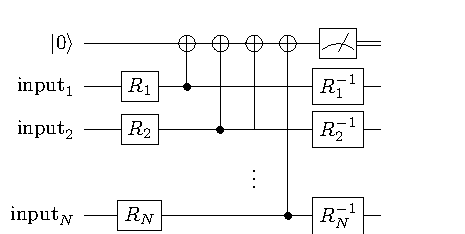
\includegraphics[width=0.45\linewidth]{figs/errormit/em-sym-ancilla-bulk-1.pdf}
    }
    \subfloat[]{
        \label{fig:em-sym-ancilla-bulk-2}
        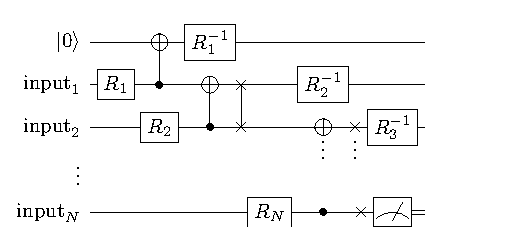
\includegraphics[width=0.45\linewidth]{figs/errormit/em-sym-ancilla-bulk-2.pdf}
    }\\
    \subfloat[]{
        \label{fig:em-sym-ancilla-bulk-mid-1}
        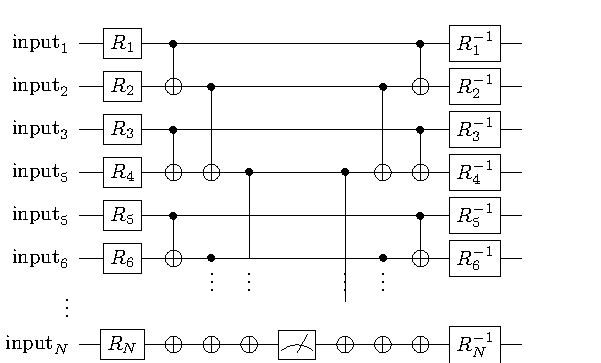
\includegraphics[width=0.45\linewidth]{figs/errormit/em-sym-ancilla-bulk-mid-1.pdf}
    }
    \subfloat[]{
        \label{fig:em-sym-ancilla-bulk-mid-2}
        \raisebox{10pt}{  % raise this figure to align better with the figure to the left
            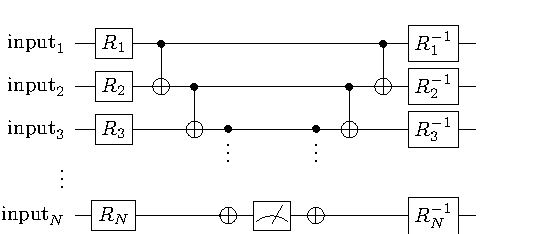
\includegraphics[width=0.45\linewidth]{figs/errormit/em-sym-ancilla-bulk-mid-2.pdf}
        }
    }
    \caption{Four different circuits that achieve the same bulk symmetry verification 
    (Sec.~\ref{sec:mit-symmetry-verification}) with different hardware requirements (adapted from \citet{bonet-monroigLowcostErrorMitigation2018}).
    In \protect\subref{fig:em-sym-ancilla-bulk-1} and \protect\subref{fig:em-sym-ancilla-bulk-2}, 
    an ancilla qubit initialized in state $\ket{0}$ is required for measuring the symmetry.
    In \protect\subref{fig:em-sym-ancilla-bulk-mid-1} and \protect\subref{fig:em-sym-ancilla-bulk-mid-2},
    the quantum computer should be able to perform a mid-circuit measurement.
    In all four circuits, the rotation gates $\{R_i\}$ perform a basis transformation such that
    the symmetry operator is equivalent to the qubit parity operator in the transformed basis.
    }
    \label{fig:mit-bulk-sym}
\end{figure}

\paragraph{Symmetry verification by post-processing:}
Verifying the symmetry $\hat{S}$ of a quantum state $\rho$ projects the state into $\rho_s$, which lies within the eigenspace of the symmetry operator with the desired valued $s$. Subsequently, an observable $\hat{O}$ is measured on the projected state,
giving a measured outcome $\mathrm{Tr}[\hat{O} \rho_s]$.
When both $\hat{S}$ and $\hat{O}$ are members of the Pauli group, it was shown \cite{bonet-monroigLowcostErrorMitigation2018} that 
\begin{equation}
    \operatorname{Tr}\left[\hat{O} \rho_{s}\right] =
    \frac{\operatorname{Tr}[\hat{O} \rho]+s \operatorname{Tr}[\hat{O} \hat{S} \rho]}{1+s \operatorname{Tr}[\hat{S} \rho]}.
\end{equation}
Therefore, the effect of symmetry verification, in this case, can be achieved with measurement outcomes of observables $\hat{O}$, $\hat{S}$, and $\hat{O}\hat{S}$. All three observables can be obtained as part of the measurements that in any case must be performed as part of the VQE optimization process.
Therefore, we can achieve symmetry verification without measuring the symmetry operator $\hat{S}$ and post-selecting the measured number. This adds one more measured observable ($\hat{O}\hat{S}$) per Pauli observable, and one more
measured observable $\hat{S}$ overall. This kind of symmetry verification is identical to a specific form of the quantum subspace expansion~\cite{bonet-monroigLowcostErrorMitigation2018}, where the excitation operators include the identity operator and the symmetry operator $\hat{S}$.

\subsection{Extrapolation based methods}
\label{sec:mit-extra}

Extrapolation methods are based on the simple idea that the measurement result $\langle \hat{O} \rangle$ on a quantum computer is affected by the strength of the noise on the device, i.e. $\langle \hat{O} \rangle= \langle \hat{O} \rangle( \varepsilon )$, where $\varepsilon$ characterizes the noise strength of the device. Therefore, using the data $\{ \langle \hat{O} \rangle (\varepsilon _{i})\}_{i\in \mathbb{N}}$ for the expectation value under several noise strength $ \{\varepsilon _{i}\}$, we can construct a mathematical model $ \langle \hat{O} \rangle ( \varepsilon |\alpha )$ describing $ \langle \hat{O} \rangle ( \varepsilon )$, where $\alpha =\{\alpha _{k}\}$ are the set of parameters parameterizing the model used for extrapolation. We can then use the same mathematical model to predict the error-free expectation value $ \langle \hat{O} \rangle_{\mathrm{exact}} \equiv \langle \hat{O} \rangle (0) \approx \langle \hat{O} \rangle ( \varepsilon =0|\alpha )$. We denote by $\varepsilon_{0}$ the smallest noise strength of the quantum computer that can be achieved by hardware engineering, i.e. $\varepsilon _{i} \geqslant \varepsilon _{0}$ for all $i\in \mathbb{N}$. Of course, on a noiseless quantum computer we would have $\varepsilon_{0}=0$, which is not a realistic assumption. Hence, $ \langle \hat{O} \rangle ( \varepsilon _{0})$ denotes the measurement outcome that would be achieved on the quantum computer without any error mitigation technique.

This method brings the additional overhead of the extra circuit executions required to obtain $\{ \langle \hat{O} \rangle ( \varepsilon _{i})\}$ at different noise levels. It also potentially add noise coming from the adjustment of the noise strength $\varepsilon$.

Care should be taken regarding implementing this method as part of a VQE algorithm: one may model the overall energy $E$ as $E=E(\varepsilon|\alpha)$, but we argue here that it is more practical to model each Pauli observable separately. That is, each Pauli observable measured separately should be modeled with an independent $ \langle \hat{O} \rangle (\varepsilon|\alpha)$.
The reason is that the difference in noise from measuring different Pauli observables is a result of the different circuits required to rotate the state in the desired measurement basis. While this is likely insignificant for naive measurements of all Pauli observables, it becomes very relevant when grouping strategies relying on general commutativity of the Pauli observables are introduced (see Sec.~\ref{sec:pauli_grouping}), since the basis rotation circuit depth scales as $\mathcal{O}(N^2)$ \cite{Gokhale2019_long}. 
It is worth pointing out that the parallel implementation for the VQE (as discussed in Sec. \ref{sec:parallelization}) also benefits from model fitting for each different hardware on which measurements are performed,
especially when the noise characteristics vary across the hardware used.
The effectiveness of extrapolation methods therefore depends on the ability to characterize and systematically increase the noise strength parameter $\varepsilon $ (Sec. \ref{sec:mit-increase_noise}), and on the soundness of the mathematical model $\langle \hat{O} \rangle( \varepsilon |\alpha )$ (see Sec. \ref{sec:mit-noise_model}).

\subsubsection{Method to systematically increase the noise}\label{sec:mit-increase_noise}

\paragraph{Re-scaling method}
This method, proposed originally by Temme \textit{et al.} \cite{temmeErrorMitigationShortDepth2017}, can achieve an effective scaling of the noise strength by rescaling the Hamiltonian $H_{\mathrm{QPU}}$ (here we are referring to the Hamiltonian driving the action of the quantum circuit on the initial state, rather than the Hamiltonian of the quantum chemistry problem we are trying to solve). The dynamics on a quantum computer
can be described by the master equation
\begin{equation}
    \partial _{t} \rho (t)=-i[\hat{H}_{\mathrm{QPU}}(t),\rho (t)]+\varepsilon _{0}\mathcal{L} [\rho (t)],
\end{equation}
where the term $\varepsilon _{0}\mathcal{L} [\rho (t)]$ represents the noise. An initial quantum state $\rho(0)$ is evolved under
the Hamiltonian $\hat{H}_{\mathrm{QPU}}(t)$ for a period of time $T$ to the state $\rho_{\varepsilon_0}$ where $\varepsilon_0$ characterize the noise strength of the quantum computer. Another copy of the same initial state is evolved under a different Hamiltonian $\hat{H}_{\mathrm{QPU}}(t/c)/c$ for a longer period of $cT$, resulted in another state $\rho_{c\varepsilon_0}$. Then, assuming the noise $\mathcal{L}$ is independent of time $t$ and of the Hamiltonian, one has
\begin{equation}
    \rho _{c\varepsilon_0} -\rho _{\varepsilon_0} =c \varepsilon _{0}\mathcal{L}.
\end{equation}
Therefore one can achieve an effective rescaling of the expectation value, resulting in $ \langle \hat{O} \rangle (\varepsilon=c \varepsilon _{0} )- \langle \hat{O} \rangle (\varepsilon=\varepsilon_0)=c \varepsilon _{0}\operatorname{Tr}[\hat{O}\mathcal{L}]$.
This scaling modifies the Hamiltonian on quantum computers directly and therefore requires precise control of the device, which has been demonstrated by the hardware team in \citet{kandalaErrorMitigationExtends2019}.
However, the recently proposed OpenPulse specification~\cite{mckayQiskitBackendSpecifications2018} allows a more
platform-independent way to control the underlying hardware which
has been used to implement this error boosting method  \cite{garmonBenchmarkingNoiseExtrapolation2020}.

\paragraph{Pauli Twirling}
Li and Benjamin \cite{liEfficientVariationalQuantum2017} propose that one can boost the physical error rate to any desired value by randomly applying Pauli gates before and after a Clifford entangling two-qubit gate, and then randomly generating additional Pauli gates after the twirled two-qubit gates. %(details can be found in \citet{liEfficientVariationalQuantum2017}).

\paragraph{Inserting CNOT gates}
\label{sec:mit-cnot-boosting}
\newcommand{\ncnot}{\ensuremath{J_\mathrm{exact}}}
Refs.~\cite{dumitrescuCloudQuantumComputing2018, heResourceEfficientZero2020} showed that when every CNOT gate is replaced by $j$ consecutive CNOT gates ($j$ should be an odd number), the measurement outcome $\langle \hat{O} \rangle(j)$ depends on $j$ by
\begin{equation}
    \label{eq:mit-insert-cnot-r}
    \langle \hat{O} \rangle(j)=\langle \hat{O} \rangle_{\mathrm{exact}} +kj+\mathcal{O}\left(\left( j\sum _{i=1}^{\ncnot} \varepsilon _{i}\right)^{2}\right) ,
\end{equation}
where $\langle \hat{O} \rangle_{\mathrm{exact}}$ is the exact measurement outcome when there is no noise, $\varepsilon _{i}$ characterizes the noise strength of the $i$-th CNOT gate, $k$ is the parameter characterizing the noise strength, and $\ncnot$ is the number of CNOT gates in the original circuit. In this model, it is assumed that the noise is dominated by the two-qubit depolarizing noise on the CNOT gates, and all other forms of error are considered negligible. The extrapolation method can therefore be used for extrapolating the case of $j=0$.

This method becomes problematic when there are a large number of CNOT gates in the original circuit, each of which needs to be replaced by $j$ CNOT gates. Eq.~(\ref{eq:mit-insert-cnot-r}) means that errors in higher orders of $j$  quickly overshadow lower-order contributions used for modeling the error. % comment: see specifically Eq(26) in the original paper. 

As a solution, \citet{heResourceEfficientZero2020} provides an approach, which is appropriate for large numbers of CNOT gates. Instead of replacing each CNOT with $r$ CNOT gates, the proposal is to replace the $i$-th CNOT gate with $j_{i}$ CNOT gates, where $(j_i - 1)/2 \sim \mathrm{Poisson}( v)$, a Poisson distribution with mean $v$. That is, the number of additional CNOT gates is sampled each time from the Poisson distribution. As a result, Eq.~(\ref{eq:mit-insert-cnot-r}) is slightly changed to
\begin{equation}
    \label{eq:mit-insert-cnot-v}
    \langle \hat{O} \rangle( v) =\langle \hat{O} \rangle_{\mathrm{exact}} +(1+2v) k +\mathcal{O}\left(\left((1+2v)\sum_{i=1}^{\ncnot}\right)^{2}\right) .
\end{equation}
Using this adjustment, the circuit is run for different values of $v$ to extrapolate to the case of $v=-1/2$. Errors in the quantum computer can be mitigated by extrapolating from measurement outcomes $\langle \hat{O} \rangle$ corresponding to different values of $j$ (Eq.~\ref{eq:mit-insert-cnot-r}) or $v$ (Eq.~\ref{eq:mit-insert-cnot-v}) using a linear model (Sec.~\ref{sec:mit-poly-model}). In particular, $v$ can be any positive number chosen such that $1+2v$ is close to $1$, making the second method more noise friendly than the first method, where $j$ can only take integer values.

\paragraph{Unitary folding:}
This method is similar to the CNOT insertion method mentioned above. Instead of inserting CNOT gates,
\citet{giurgica-tironDigitalZeroNoise2020} proposes that one can insert only gates from the original circuit to boost the error rate. In this method, named \textit{unitary folding}, one assumes a unitary circuit $U$ is made from several layers $\{U_i\}_{i=1}^d$ of quantum gates
\begin{equation}
    U = U_d \cdots U_2 U_1,
\end{equation}
where $d$ is the number of layers. To boost the error, $U$ is transformed into an equivalent circuit
\begin{equation}
    U_{\mathrm{folded}} =U(U^{\dagger } U)^{L_{1}} U_{l_{L_{2}}}^{\dagger } U_{l_{L_{2} -1}}^{\dagger } \cdots U_{l_{1}}^{\dagger } U_{l_{1}} \cdots U_{l_{L_{2} -1}} U_{l_{L_{2}}} ,
\end{equation}
where $U$ has been \textit{folded} $2L_2+1$ times, and an additional subset $\{l_1,l_2,\cdots, l_{L_2}\}$ ($L_2<d$) of the $d$ layers is chosen to boost the error even further. There is no particular rule as to how this subset should be chosen. However, these additional gates give us additional freedom to control the noise strength. One can define $\lambda$ as the ratio of layers in the folded circuit over the original circuit
\begin{equation}
    \lambda = \frac{(2L_1+1)d + 2L_2}{d} = 2L_1+1 + \frac{2L_2}{d}.
\end{equation}

Form this point, $\lambda$ can be systematically increased with a step size of $2/d$, giving granular control of this noise parameter. Assuming a depolarizing noise model on all qubits, the measurement output of the folded circuit has the form
\begin{equation}
    \langle \hat{O} \rangle(\lambda) = \langle \hat{O} \rangle_{\mathrm{exact}} + b \varepsilon^\lambda,
\end{equation}
where $b$ and $\varepsilon$ are coefficients that are determined from extrapolating from the measured data. Therefore, extrapolation to the case of $\lambda=0$ can give the desired error-free measurement outcome.

\paragraph{Multi-parameter noise model:}
It is, in general, more realistic to characterize the noise of a quantum computer by multiple parameters, such as the  times $T_1$ and $T_2$ (see Sec.~\ref{sec:mit-noise-relaxation}), which are usually used as figure of merits for quantum computers. In this case, the noise parameter $\varepsilon$ becomes a vector
$\varepsilon = (\varepsilon^{(1)},\cdots, \varepsilon^{(l)},)$ of $l$ different noise parameters.
\citet{ottenRecoveringNoisefreeQuantum2019} discusses an interesting scenario where $T_1$ and $T_2$ are
estimated and used to build a model that recovers the population in state $\ket{1}$.
Although we have not seen a method that systematically controls errors on multiple noise parameters,
we note that all modeling methods discussed below may be generalized to this multi-parameter case.

\subsubsection{Modeling the noise and extrapolating from measured data} \label{sec:mit-noise_model}

Once a suitable technique has been developed to artificially increase the noise in the device, one can turn towards finding a model to extrapolate the data to obtain a better approximation of the true expectation value.  A general formulation of the extrapolation can be made: given the model $\langle \hat{O} \rangle(\varepsilon|\alpha)$ and several measurement outcomes $\langle \hat{O} \rangle(\varepsilon_i)$, an optimal coefficient $\alpha^*$ can be found by optimizing function $f(\alpha)$, which measures the squared error between prediction $\langle \hat{O} \rangle(\varepsilon_i|\alpha)$ and the measurement outcome $\langle \hat{O} \rangle(\varepsilon_i)$
\begin{equation}
    \label{eq:mit-model-square-loss}
    f(\alpha) = \sum_i |\langle \hat{O} \rangle(\varepsilon_i) - \langle \hat{O} \rangle(\varepsilon_i|\alpha)|^2.
\end{equation}
This method is very common in data analysis, and is often used in regression techniques (for further details, see Ref. \cite{goodfellowDeepLearning2016}). 

\paragraph{Linear/Polynomial model:} \label{sec:mit-poly-model}
In this model $\langle \hat{O} \rangle( \varepsilon |\alpha )$ can be generalized to
\begin{equation}
    \label{eq:mit-linear-1}
    \langle \hat{O} \rangle( \varepsilon |\alpha ) -\langle \hat{O} \rangle_{\mathrm{exact}} =\sum ^{K}_{k=0} \alpha _{k} \varepsilon ^{k} + \mathcal{O}(\varepsilon^{K+1}),
\end{equation}
which was shown to be valid in \citet{temmeErrorMitigationShortDepth2017}, when assuming that the noise on quantum computer is small enough, such that the residual noise $\langle \hat{O} \rangle( \varepsilon ) -\langle \hat{O} \rangle( \varepsilon |\alpha ) =\mathcal{O}( \varepsilon ^{K+1})$.
This function was also shown to characterize noise correctly when inserting additional identity gates into the quantum circuits, see Sec.~\ref{sec:mit-cnot-boosting}.

Having obtained $\langle \hat{O} \rangle(\varepsilon _{i} )_{i=0}^{L}$, where $L+1$ is the number of measurement outcomes we obtained for $L+1$ different values of $\varepsilon _{i}$, we mention two methods to extrapolate an approximation to the exact measurement outcome $\langle \hat{O} \rangle_{\mathrm{exact}}$. The first method is called Richardson extrapolation~\cite{liEfficientVariationalQuantum2017,temmeErrorMitigationShortDepth2017}, and can be applied when $L=K$. Here, one rewrites Eq.~(\ref{eq:mit-linear-1}) as
\begin{equation}
    \label{eq:Richardson_eq1}
    \langle \hat{O} \rangle(c_{i} )=\langle \hat{O} \rangle_{\mathrm{exact}} +\sum _{k=0}^{K} \alpha _{k}( c_{i} \varepsilon _{0})^{k} +\mathcal{O} (c_{i}^{K+1} ),
\end{equation}
where $c_{i} =\varepsilon _{i} /\varepsilon _{0}$ is the ratio of the noise strength of different cases relative to the reference value $\varepsilon _{0}$. Next, one seeks a series of combination coefficients $\beta _{i}$ such that
\begin{equation}
    \begin{split}
        \label{eq:mit-richardson-1}
        \sum _{i} \beta _{i} \langle \hat{O} \rangle( c_{i}) & =\langle \hat{O} \rangle_{\mathrm{exact}} ,
    \end{split}
\end{equation}
for any $\varepsilon_{0}$, ignoring the higher order terms $\mathcal{O} (\varepsilon_0^{N+1} )$ in Eq.~\ref{eq:Richardson_eq1}. That is, one considers Eq.~(\ref{eq:mit-richardson-1}) as an equivalence of two polynomials in $\varepsilon _{0}$, leading to the conditions
\begin{equation}
    \begin{split}
        \sum _{i} \beta _{i} & =1,\\
        \sum _{i} \beta _{i} c_{i}^{k} & =0,\ k=1,2,\cdots K,
    \end{split}
\end{equation}
which admit the solution
\begin{equation}
    \begin{split}\label{eq:mit-poly-beta}
        \beta _{i} & =\prod _{k\neq i}\frac{c_{k}}{c_{k} - c_{i}} .
    \end{split}
\end{equation}
It is worth noting that more explicit formulae for the constants $c_i$ can be obtained assuming depolarizing noise in the CNOT-insertion based error boosting method~\cite{heResourceEfficientZero2020}, see Sec.~\ref{sec:mit-cnot-boosting}.

The second method is a simple extension of the linear regression technique commonly found in machine learning \cite{hastie2015statistical}, which we already mentioned above (Eq.~\ref{eq:mit-model-square-loss}). Here, the optimization can be furthered simplified. One first rewrites Eq.~(\ref{eq:mit-linear-1}) into a matrix form by defining
\begin{equation}
    \begin{split}
        \label{eq:mit-poly-regression}
        A & =\begin{pmatrix}
            1      & \varepsilon _{0} & \cdots & \varepsilon _{0}^{K} \\
            1      & \varepsilon _{1} & \cdots & \varepsilon _{1}^{K} \\
            \vdots & \vdots           &        & \vdots               \\
            1      & \varepsilon _{L} & \cdots & \varepsilon _{L}^{K}
        \end{pmatrix} ,\\
        X & =( \langle \hat{O} \rangle_{exact} ,\alpha _{1} ,\cdots ,\alpha _{K})^{T} ,\\
        Y & =( \langle \hat{O} \rangle( \varepsilon _{0}) ,\langle \hat{O} \rangle( \varepsilon _{1}) ,\cdots ,\langle \hat{O} \rangle( \varepsilon _{L}))^{T} ,\\
        f( X) & =( AX-Y)^{T}( AX-Y) ,
    \end{split}
\end{equation}
where the cost function $f$ measures the squared difference between the measurement outcome $Y$ and the prediction $AX$ (i.e. $\langle \hat{O} \rangle( \varepsilon _{i} |\alpha )$). The minima of $f$ (which contains the desired $\langle \hat{O} \rangle_{\mathrm{exact}}$) can be obtained using the equation \cite{hastie2015statistical}
\begin{equation}
    \begin{split}
        X^{*} & =\argmin_{X} \ f( X) =\left( A^{T} A\right)^{-1} A^{T} Y,
    \end{split}
\end{equation}
when $A^{T} A$ is not singular. Note that one often controls the ratio $c_{i} =\varepsilon _{i} /\varepsilon _{0}$, and the method works in the same manner by replacing $\varepsilon _{i}$ with $c_{i}$ in Eq.~(\ref{eq:mit-poly-regression}).

Here we compare the two methods. The Richardson extrapolation coincides with the second minimization method when $K=L$. This can be seen by noticing that $A$ has the form of a Vandermonde matrix and its determinant when $K=L$ is $\prod _{0\leqslant i< j\leqslant K}( \varepsilon _{j} -\varepsilon _{i})$, which is always invertible when the $\varepsilon _{i}$ have distinct values. However, although it may be less interesting to consider the case when $K>L$ when there are insufficient measurement samples to fix the free parameters in our model Eq.~(\ref{eq:mit-linear-1}), we argue here that the $K<L$ case is interesting; this uses a polynomial of order $K$, which is smaller than $L$, the number of measurement samples. The argument is as follows: although when $K=L$ we may obtain a solution $\alpha $ such that each measurement outcome $M( \varepsilon _{i})$ could be exactly predicted by our model $M( \varepsilon |\alpha )$, a model with higher-order polynomials is more sensitive to statistical fluctuations \cite{giurgica-tironDigitalZeroNoise2020} and generally does not perform well for predicting new values. Similar arguments could be found in the machine learning literature under the topic of \textit{over-fitting }\cite{goodfellowDeepLearning2016}. In this case, the second method is also compatible with techniques addressing the over-fitting problem, such as the Lasso regression\cite{hastie2015statistical}.

Finally, it is very important to note that extrapolation based on this model increases the cost of the VQE algorithm, possibly prohibitively. For each Pauli observable evaluation, the required circuit evaluation is multiplied by the size of data used to fit the model, and the variance of the observable is also increased by a factor $\gamma$. When the Richardson extrapolation is used, or when the matrix $A$ in Eq.~(\ref{eq:mit-poly-regression}) is a square and non-singular matrix, $\gamma$ can be derived analytically \cite{suguru2019a,temmeErrorMitigationShortDepth2017} as
\begin{equation}\label{eq:mit-poly-variance-amplification}
    \gamma = \sum_i \beta_i^2,
\end{equation}
with $\beta_i$ as in Eq.~(\ref{eq:mit-poly-beta}).

\paragraph{Exponential model:} \label{sec:mit-exp-model}
For a deep circuit, it is natural to expect that the error dominates the quantum computation exponentially fast.
\citet{endoPracticalQuantumError2018} demonstrated this in a simple example,
where a quantum circuit consisting of $J$ noisy gates is executed on a noisy quantum computer. It assumes that the noise
on the $i$-th identity gate $\mathcal{E}_i$ can be modeled by a simple error model of the form
\begin{equation}
    \mathcal{E}_i(\rho) = (1-\varepsilon) \rho + \varepsilon \mathcal{\mathcal{E}'}_{i} (\rho).
\end{equation}
An example is the depolarizing noise, where $\mathcal{E'}_i(\rho) \propto \unit$. With this assumption,
the overall noise effect $\prod_i \mathcal{E}_i$, when $J$ is large, can be approximated by
\begin{equation}
    \prod_i \mathcal{E}_i \approx e^{-J\varepsilon}  \sum_{k=0}^{J} \frac{(J\varepsilon)^k}{k!} \mathcal{X}_k,
\end{equation}
where $\mathcal{X}_k$ contains contributions of $\mathcal{E'}$ applied $k$ times towards the product. In order to fit an exponential noise extrapolation model, one can re-write $\langle \hat{O} \rangle( \varepsilon |\alpha )$ as
\begin{equation}
    \label{eq:mit-exp-1}
    \langle \hat{O} \rangle( \varepsilon |\alpha ) -\langle \hat{O} \rangle_{\mathrm{exact}} =A\exp( -J \varepsilon ).
\end{equation}
\citet{endoPracticalQuantumError2018} gives an explicit formula for $\langle \hat{O} \rangle( 0)$, computable with prior knowledge of $\langle \hat{O} \rangle( \varepsilon _{0})$ and $\langle \hat{O} \rangle( k\varepsilon _{0})$,
\begin{equation}
    \label{eq:mit-exp-2}
    \langle \hat{O} \rangle(0) = \frac{k e^{J \varepsilon}\langle \hat{O}\rangle(\varepsilon)-e^{J k \varepsilon}\langle \hat{O}\rangle(k \varepsilon)}{k-1}.
\end{equation}
Furthermore, one can combine the exponential model with the polynomial model into a poly-exponential extrapolation \cite{giurgica-tironDigitalZeroNoise2020}, where the noise model is
\begin{equation}
    \langle \hat{O} \rangle( \varepsilon |\alpha ) = A + B \exp(\mathrm{poly}(\varepsilon)).
\end{equation}
Here the degree of the polynomial in $\varepsilon$ needs to be chosen by experience, and the coefficients can be obtained with the minimization method mentioned at the beginning of this section. Giurgica-Tiron \textit{et al.} \cite{giurgica-tironDigitalZeroNoise2020} demonstrate that this method successfully mitigates errors resulting from quantum circuit execution, however, they do not compare with other extrapolation methods in terms of cost and benefits. 

Extrapolation based on this model similarly increases the cost of the VQE  algorithm.  For each Pauli string evaluation, the number of circuit repetitions is multiplied by the size of data, and as above, the variance of the observable is also increased by a factor $\gamma$.  For a simple exponential model in Eq.~(\ref{eq:mit-exp-2}), $\gamma$ can be derived analytically as \cite{suguru2019a}
\begin{equation}
    \gamma = \frac{k^{2} \exp(2\varepsilon J)+\exp(2 k \varepsilon J )}{(k-1)^{2}},
\end{equation}
assuming the variance of $\langle \hat{O} \rangle( \varepsilon _{0})$ and $\langle \hat{O} \rangle( k\varepsilon _{0})$ are equal.
One can note that the variance in this exponential model tends to be significantly larger than for the polynomial model. %However, it has been shown to result in more accurate predictions. \cite{endoPracticalQuantumError2018}.
However, it has been shown~\cite{endoPracticalQuantumError2018} that if enough sampling is affordable, this exponential model gives more accurate prediction of the exact measurement outcome than the polynomial model.
The polynomial model can be seen as an approximation to this exponential model when the noise
$\varepsilon$ is not very high.

% General plan: move the example into the appendix.
\subsection{Probabilistic error cancellation}
\label{sec:mit_pec}
In Probabilistic error cancellation (PEC) \cite{temmeErrorMitigationShortDepth2017,endoPracticalQuantumError2018},
quantum circuits are actively modified with the overall goal of inverting the impact of noise on a quantum computer. Mathematically, the estimated ideal measurement value $\langle \hat{O} \rangle$ is obtained as
\begin{equation}
    \label{eq:mit-pec-1}
    \langle \hat{O} \rangle_{\mathrm{PEC}} =\sum _{i} q_{i} \langle \hat{O} \rangle_{\mathrm{PEC},i} \ ( q_{i} \in \mathbb{R}),
\end{equation}
where each measurement value $\langle \hat{O} \rangle_{\mathrm{PEC},i}$ corresponds to a different, slightly modified, quantum circuit. Specifically,
given a quantum circuit $U=\prod_k U_k$,
one finds weights $q_{i_k}$ and operations on quantum computer $B_{i_k}$ such that
\begin{equation}
    U_k = \sum_{i_k} q_{i_k} B_{i_k},
\end{equation}
and hence overall
\begin{equation}\label{eq:mit-pec-cor-all-decomp}
U = \prod_k \left(\sum_{i_k} q_{i_k} B_{i_k}\right) 
= \sum_{i_1,i_2,\cdots} \prod_k q_{i_k} B_{i_k}.
\end{equation}
Here the weights $\prod_k q_{i_k}$ are used as the coefficient $q_i$ in Eq.~(\ref{eq:mit-pec-1}),
where $i$ is an abbreviation of the many indices $i_1,i_2,\cdots$.
We provide an example correcting single-qubit gates under the depolarizing noise in Appendix~\ref{sec:mit-pec-toy-example}.

One expects the terms in the summation to explode exponentially
with respect to the depth of the circuit.
Therefore, it helps to implement Eq.~(\ref{eq:mit-pec-1}) probabilistically.
To do this, one rewrites Eq.~(\ref{eq:mit-pec-1}) as
\begin{equation}
    \label{eq:mit-pec-5}
    \begin{split}
        \langle \hat{O} \rangle_{\mathrm{PEC}} & =\gamma _{\mathrm{PEC}}\sum _{i}\mathrm{sgn}( q_{i}) P_{\mathrm{PEC}} \langle \hat{O} \rangle_{\mathrm{PEC} ,i} ,\\
        \gamma _{\mathrm{PEC}} & =\sum _{i} |q_{i} |,\ P_{\mathrm{PEC}} =\frac{| q_{i}| }{\gamma _{\mathrm{PEC}}} .
    \end{split}
\end{equation}
Here $\mathrm{sgn}( q_{i})$ is the sign of $q_{i}$, and $P_{\mathrm{PEC}}$ is a proper probability distribution normalized by the constant $\gamma _{\mathrm{PEC}}$. Eq.~(\ref{eq:mit-pec-5}) provides a probabilistic implementation of the summation in Eq.~(\ref{eq:mit-pec-1}). That is, we could sample from all the modified circuits according to the distribution $P_\mathrm{PEC}$ and execute them. The overall measurement $\langle \hat{O} \rangle_{\mathrm{PEC}}$ can be estimated by adding measurement result $\langle \hat{O} \rangle_{\mathrm{PEC} ,i}$ from each circuit weighted by the factor $\gamma _{\mathrm{PEC}}\mathrm{sgn}( q_{i}) P_{\mathrm{PEC}}$. When the number of modified circuits is large, it is more practical to estimate \ $\langle \hat{O} \rangle_{\mathrm{PEC}}$ using this probabilistic implementation. For this reason, this mitigation technique is called \textit{probabilities error cancellation}.
In the literature \cite{endoPracticalQuantumError2018, temmeErrorMitigationShortDepth2017} pairs of weights $q_{i_k}$ and operations $B_{i_k}$ are considered as a \textit{quasi-probability representation} of $U_k$, $q_{i_k}$ or $q_i$. These are referred to as the \textit{quasi-probability weights}, and incidentally the mitigation method is called the \textit{quasi-probability method}.

Before discussing the quasi-probability representation and its construction, we first discuss its cost. Although the number of noisy circuits in a quasi-probability representation of the ideal circuit $U$ grows exponentially with respect to the depth of the circuit (Eq.~\ref{eq:mit-pec-cor-all-decomp}),
with the probabilistic implementation the cost of PEC only depends on how fast the probabilistic sampling converges,
i.e. the variance of $\langle \hat{O} \rangle_{\mathrm{PEC}}$. Assuming that the measurement outcomes of different circuits $\langle \hat{O} \rangle_{\mathrm{PEC,i}}$ are independent and that their variance can be bounded by $1$
(which applies to the Pauli observable of interest in the VQE algorithm), the variance of $\langle \hat{O} \rangle_{\mathrm{PEC}}$ could be bounded by $\gamma_{\mathrm{PEC}}^2$.

Now we detail how the modified circuits are constructed in the general case \cite{endoPracticalQuantumError2018,strikisLearningbasedQuantumError2020,Takagi2021OptimalResource}. There are several approaches to this problem, and here we mention two important methods. The first constructs modified circuits using tomography data from quantum computers, the second constructs modified circuits based on data from a quantum computer and a given ansatz structure.

\paragraph{Tomography based method  \cite{endoPracticalQuantumError2018}:} Given a circuit $U$ that consists of unitary gates $U=\prod _{k} U_{k}$, we assume that the effect of noise on each unitary gate can be characterized (by tomography) as $\mathcal{U}_{k,\mathrm{noisy}} =\mathcal{N}_{k} \circ \mathcal{U}_{k}$, and that is there is no correlation between errors on quantum gates acting on different qubits (spatial correlation) or different time steps (temporal correlation).
Here $\mathcal{U}_k$ represents the quantum channel corresponding to the unitary gate $U_k$, and is typeset in an italic font to emphasize it being a quantum channel.
From there, one must find pairs of quasi-probability weights $q_{i,k}$ and quantum operations $\mathcal{B}_{i,k}$ (which are not necessarily unitary gates) such that
\begin{equation}
    \label{eq:mit-pec-6_3}
    \mathcal{U}_{k} =\sum _{i} q_{i,k} \mathcal{B}_{i,k} \mathcal{U}_{k,\ \text{noisy}},
\end{equation}
and overall the quantum channel $\mathcal{U}$ corresponding to the unitary gate $U$ is expressed as
\begin{equation}
    \label{eq:mit-pec-7}
    \mathcal{U} =\sum_{k,i} q_{i,k} \mathcal{B}_{i,k} \mathcal{U}_{k,\ \text{noisy}} .
\end{equation}
To find such $\mathcal{U}$, one obtains the gate-wise noise model $\mathcal{N}_k$ for each $k$ using tomography. Then, a different formalism to describe the quantum process $\mathcal{N}_k$ named Pauli transfer matrix formalism is used to obtain the (non-physical) channel $\mathcal{N}^{-1}_k$, described by a linear summation of several basis operations $\{\mathcal{B}'_{i}\}$. We refer the readers to Ref.~\cite{endoPracticalQuantumError2018} for implementation details.

\paragraph{Learning based method:}

This method, proposed by Strikis \textit{et al.} \cite{strikisLearningbasedQuantumError2020} assumes that single-qubit errors are negligible, and can be applied to quantum circuits having a specific layer-wise structure.
In each layer of these quantum circuits, single qubit gates are followed by Clifford multi-qubit gates. Pauli gates are inserted in between single qubits gates and Clifford multi-qubit gates to mitigate errors (see
Fig.~\ref{fig:mit-learning-PEC-setup}). Specifically, we denote all the Clifford multi-qubit gates collectively by $\mathbf{G}$ (called \textit{frame gates} in the original paper), all single qubits in the unmodified circuit collectively by $\mathbf{R}$, and all the additional inserted Pauli gates by $\mathbf{P}$. To mitigate the error, different combinations of single qubit Pauli gates are inserted, labeled as $\mathbf{P}=(P_1,P_2,\cdots )$, resulting in different quantum circuits. Each of these gives a measurement value labeled by $\langle \hat{O} \rangle(\mathbf{R},\mathbf{P})$. The overall mitigation result $\langle \hat{O} \rangle^{\mathrm{mit}}( \mathbf{R}, q)$ is
\begin{equation}
    \label{eq:mit-pec-l}
    \langle \hat{O} \rangle^{\mathrm{mit}}( \mathbf{R},q) =\sum _{\mathbf{P}} q( \mathbf{P}) \langle \hat{O} \rangle( \mathbf{R},\mathbf{P}),
\end{equation}
where $q:\mathbf{P}\mapsto q( \mathbf{P}) \in \mathbb{R}$ associates a specific weight to a specific combination $\mathbf{P}$. Eq.~(\ref{eq:mit-pec-l}) resembles the quasi-probability formula Eq.~(\ref{eq:mit-insert-cnot-r}) closely, except for the structure of the circuit, and the procedure to modify the circuits. To find the appropriate weights $q(\mathbf{R})$, Strikis \textit{et al.} \cite{strikisLearningbasedQuantumError2020} define a loss function
\begin{equation}
    \label{eq:mit-pec-lcost}
    \mathrm{Loss}( q) =\frac{1}{|\mathbb{T} |}\sum _{\mathbf{R}\in \mathbb{T}} |\langle \hat{O} \rangle^{\mathrm{mit,qpu}}( \mathbf{R},q) -\langle \hat{O} \rangle^{\mathrm{mit,sim}}( \mathbf{R}) |^2,
\end{equation}
where the single qubit gates in the original circuit are substituted by single qubit gates in the set $\mathbb{T}$, called the training set. The substituted circuits are simulated to obtain an exact simulation result $\langle \hat{O} \rangle^{\mathrm{mit,sim}}(R)$. Pauli gates are inserted in the manner specified in Fig.~\ref{fig:mit-learning-PEC-setup} and executed on a quantum computer to obtain the noisy result $\langle \hat{O} \rangle^{\mathrm{qpu,noisy}}( \mathbf{R},q)=\sum_\mathbf{P} q(\mathbf{P}) \langle \hat{O} \rangle(\mathbf{R},\mathbf{P})$.

\begin{figure}[ht]
    \centering
    $
\Qcircuit @C=1.0em @R=0.8em @!R { \\
\lstick{\ket{0}} & \gate{P_1} & \gate{R_1} & \gate{P_5} & \qw & \gate{P_9} & \gate{R_5} & \gate{P_{13}} & \multigate{1}{G_2} & \gate{P_{17}} & \gate{R_9} & \gate{P_{21}} & \meter \\
\lstick{\ket{0}} & \gate{P_2} & \gate{R_2} & \gate{P_6} & \multigate{1}{G_1} & \gate{P_{10}} & \gate{R_6} & \gate{P_{14}} & \ghost{G_2} & \gate{P_{18}} & \gate{R_{10}} & \gate{P_{22}} & \meter \\
\lstick{\ket{0}} & \gate{P_3} & \gate{R_3} & \gate{P_7} & \ghost{G_1} & \gate{P_{11}} & \gate{R_7} & \gate{P_{15}} & \multigate{1}{G_3} & \gate{P_{19}} & \gate{R_{11}} & \gate{P_{23}} & \meter \\
\lstick{\ket{0}} & \gate{P_4} & \gate{R_4} & \gate{P_8} & \qw & \gate{P_{12}} & \gate{R_8} & \gate{P_{16}} & \ghost{G_3} & \gate{P_{20}} & \gate{R_{12}} & \gate{P_{24}} & \meter 
\gategroup{2}{5}{5}{5}{2.5em}{--}
\gategroup{2}{9}{5}{9}{1em}{--}
\\
}
$
    % \includegraphics[width=0.9\linewidth]{figs/mit-learning-PEC-setup.png}
    \caption{Setup of the learning based probabilistic error cancellation method 
    (adapted from \citet{strikisLearningbasedQuantumError2020}).
    A quantum circuit is partitioned into single qubit gates $\mathbf{R}=(R_1,R_2,\cdots)$ followed by Clifford multi-qubit gates $\mathbf{G}=(G_1,G_2,\cdots)$. Additional, single qubit Pauli gates $\mathbf{P}=(P_1,P_2,\cdots )$ are inserted in between the single qubit gates and Clifford gates to mitigate errors.}
    \label{fig:mit-learning-PEC-setup}
\end{figure}

Overall, one aims to find the weights $q$ such that the loss function in Eq.~(\ref{eq:mit-pec-lcost}) is minimized. Strikis \textit{et al.} \cite{strikisLearningbasedQuantumError2020} show that if the training set $\mathbb{T}$ is chosen as the set of all Clifford circuits, and if one assumes that there exists a $q^{*}$ such that $\mathrm{Loss}\left( q^{*}\right) =0$, then
\begin{equation}
    \langle \hat{O} \rangle^{\mathrm{mit,qpu}}\left( \mathbf{R},q^{*}\right) =\langle \hat{O} \rangle^{\mathrm{exact}}\left( \mathbf{R}\right),
\end{equation}
for any set of single qubit gates $\mathbf{R}$. Here it is also assumed that the single qubit errors (i.e. errors for $\mathbf{R}$) are negligible. The quantity $\langle \hat{O} \rangle^{\mathrm{exact}}\left( \mathbf{R}\right)$ is the exact result of the original circuit without error.

% Although for general noise models the weights $q^{*}$ may not exist, the structure of Pauli gates surrounded on both sides of Clifford multi-qubit gates (see Fig.~\ref{fig:mit-learning-PEC-setup}) resembles the setup of Pauli twirling on a Clifford gate, which converts general errors into Pauli errors \cite{liEfficientVariationalQuantum2017}. Therefore we can assume the noise on the Clifford gates $\mathbf{G}$ are Pauli. While in general, it is not possible to guarantee that a set of weights  $q^{*}$ which invert the effect of noise exists, it is possible in the case of the Pauli noise model (an example is mentioned at the beginning of this section).

Although Strikis \textit{et al.} \cite{strikisLearningbasedQuantumError2020} has not discussed the optimization of the loss function $\mathrm{Loss}(q)$, it discussed in detail the approach to sampling the training set $\mathbb{T}$ and the set of all Pauli operators $\mathbb{P}$ for estimating the loss function, which might be a concern since both sets grow exponentially with respect to the number of qubits.

% One crucial step in this approach is to evaluate the loss function $\mathrm{Loss}(q)$ and optimize it. Strikis \textit{et al.} \cite{strikisLearningbasedQuantumError2020} offers no details on the optimization, but discuss in detail the approach to sampling the training set $\mathbb{T}$ and the set of all Pauli operators $\mathbb{P}$ for estimating the loss function, since the size of both sets grows exponentially with respect to the number of qubits.

\subsection{Exponential error suppression}
\label{sec:mit-ees}
This method was independently proposed in \citet{koczorExponentialErrorSuppression2021,hugginsVirtualDistillationQuantum2021}, and further developed by \citet{obrienErrorMitigationVerified2021, huoDualstatePurificationPractical2021, cai2021resourceefficient}. It is called \textit{exponential suppression by derangement} in \citet{koczorDominantEigenvectorNoisy2021}, and \textit{virtual distillation} in \citet{hugginsVirtualDistillationQuantum2021}.
For fairness, we refer to this method as exponential error suppression to highlight its ability to suppress errors exponentially. Using different circuits, all variants of this method compute the value
% paused here.

\begin{equation}
    \label{eq:ees-computed-rhon}
    \frac{\operatorname{Tr}\left[ \rho ^{\nEES} \hat{O}\right]}{\operatorname{Tr}\left[ \rho ^{\nEES}\right]},
\end{equation}
where a quantum state $\rho$ is prepared by a circuit, e.g. the ansatz circuit of VQE. Here, $\hat{O}$ can be any observable, and $\nEES$ is a free parameter that can be adjusted. The effect of calculating Eq.~(\ref{eq:ees-computed-rhon})
instead of directly $\operatorname{Tr}[\rho O]$ is that the dominant eigenvector in $\rho$ is be amplified exponentially with respect to $\nEES$. 
More precisely, from the spectral decomposition of~$\rho$
\begin{equation}
    \label{eq:ees-spectral-decomposition}
    \rho = \sum_{i} p_i \ket{\psi_i}\bra{\psi_i},
\end{equation}
where we adopt the convention that $p_i\geqslant p_{i+1}$, one can show \cite{koczorExponentialErrorSuppression2021} that
\begin{equation}
\begin{split}
    \frac{\mathrm{Tr}\left(\rho ^{\nEES} \hat{O}\right)}{\mathrm{Tr}\left( \rho ^{\nEES}\right)} 
    &= \langle \psi _{1} |\hat{O}|\psi _{1} \rangle + \mathcal{O}(Q^\nEES),
\end{split}
\end{equation}
where $Q\equiv \left(p_1^{-1} -1\right)p_2<1$.

Therefore, if one wants the difference between the contribution from the dominant eigenvector $\bra{\psi_1} \hat{O} \ket{\psi_1}$ 
and the overall calculated value to be only $\epsilon$, one needs $\nEES$ to be\cite{koczorExponentialErrorSuppression2021}:
\begin{equation}
    \nEES = \operatorname{ceil}(\ln{\frac{1}{\epsilon}} + \frac{\ln(2\,p^{-1}_2)}{\ln Q^{-1}})
\end{equation}
where $\operatorname{ceil}(x)$ gives the ceiling of $x$, i.e. the smallest integer that is greater than or equal to $x$.
The calculation of the numerator in the Eq.~(\ref{eq:ees-computed-rhon}) on a quantum computer can be achieved
with the circuit outlined in Fig.~\ref{fig:ees-controlled-D-implement}, or by several alternative methods detailed in the Appendix~\ref{sec:derangement-details}.

\begin{figure*}
    \subfloat[Example of exponential error suppression circuit for $\nEES=3$]{
        \label{fig:ees-general-circ}
        \makebox[0.5\linewidth]{
        $
\Qcircuit @C=1.0em @R=0.8em @!R { \\
\lstick{\ket{0}} & \qw & \gate{H} & \ctrl{1} & \ctrl{1} & \gate{H} & \meter & \rstick{\rightarrow\operatorname{Tr}(\rho^\nEES{} O)} \\
\lstick{\rho} & \qw & \qw & \multigate{2}{D_\nEES} & \gate{P} & \qw & \qw \\
\lstick{\rho} & \qw & \qw & \ghost{D_\nEES} & \qw & \qw & \qw \\
\lstick{\rho} & \qw & \qw & \ghost{D_\nEES} & \qw & \qw & \qw \\
}
$
        }
    }
    \subfloat[Example of derangement circuit on $\nEES$ copies of $\rho$]{
        \label{fig:ees-VD-swap-circ}
        \makebox[0.5\linewidth]{
        \resizebox{0.2\linewidth}{!}{
        $
\Qcircuit @C=1.5em @R=1.5em @!R { \\
\lstick{\rho} & \qswap & \qw & \qw & \qswap\qwx[4] & \qw \\
\lstick{\rho} & \qswap\qwx & \qswap & \qw & \qw & \qw \\
\lstick{\rho} & \qw & \qswap\qwx & \qswap\qwx[1] & \qw & \qw \\
& \vdots & & & \\
\lstick{\rho} & \qw & \qw & \qswap & \qswap & \qw \\
}
$
        }
        }
    }
    \caption{General circuits to compute the numerator in Eq.~(\ref{eq:ees-computed-rhon})
    for exponential error suppression 
    (adopted from \citet{koczorExponentialErrorSuppression2021}).
    Here for simplicity we only considered the case when $\nEES=3$,
    but the circuit could be easily generalized to arbitrary $\nEES\geq 2$.
    $D_\nEES$ is the circuit which performs a derangement on all indices $\{i_1,\cdots,i_\nEES\}$. An example of $D_\nEES$
    is shown to the right. It swaps all nearest neighbor qubits, as well as the first and the last qubit. Details on properties of $D_\nEES$ could be found in the appendix~\ref{sec:derangement-details}.
    }
    \label{fig:ees-controlled-D-implement}
\end{figure*}


To apply this method to the VQE algorithm, the mixed state $\rho$ can be prepared by the ansatz circuit $U(\boldsymbol{\theta})$
in a noisy quantum computer, and then each Pauli observable $P$ in the decomposed Hamiltonian is measured
on $\rho$ with this suppression technique. 
If the energy has been minimized, the dominant state $\ket{\psi_1}$ in $\rho$ prepared by the ansatz circuit
has energy exponentially close to the true ground state energy of the Hamiltonian.
Therefore, exponential error suppression purifies the mixed state and helps to prepare a pure eigenstate of Hamiltonian when combined with VQE.

Meanwhile, the variance of the measured quantity, when $\hat{O}$ is again also a unitary
operator, is comparable to the variance of measuring $\hat{O}$ directly. More precisely,
the number of samples $S$ required to achieve a small error $\epsilon_s^2$ in variance of estimating either the numerator or the denominator is of the order~\cite{koczorExponentialErrorSuppression2021}
\begin{equation}\label{eq:ees-variance}
    \mathcal{O}[\epsilon ^{-2(1+2f)}_{s}],
\end{equation}
where $f=\ln(p_1^{-1})/\ln(Q^{-1}))>0$, which converges to the limiting case without error mitigation method ($\mathcal{O}(\epsilon^{-2})$) as $p_1$ goes to $1$ and $p_2$ goes to $0$.

Next, we note that $\ket{\psi_1}$ is not necessarily the ideal error-free computation result $U(\boldsymbol{\theta})\ket{0}$.
Although this does not affect the VQE algorithm itself as mentioned above, 
it affects some VQE-based algorithms. 
For example, the excited state VQE algorithms (see Sec. \ref{sec:excited_states}) that measure the fidelity between 
$\ket{\psi_1}$ and other quantum states, are affected by the fact that
the inverse unitary $U(\boldsymbol{\theta})^\dagger$ no longer prepares the adjoint $\bra{\psi_1}$ from $\bra{0}$.
Although there is no known efficient solution to this problem, the infidelity between the ideal error-free computation result and $\ket{\psi_1}$, called the coherent mismatch, has been studied extensively in \citet{koczorDominantEigenvectorNoisy2021},
where it is shown that the error from coherent mismatch can be guaranteed to be smaller than the
error caused by the limitation in creating more copies (i.e. the limitation in $\nEES$).

Finally, it is important to mention that there are several methods with different advantages to compute the quantities in Eq.~(\ref{eq:ees-computed-rhon}), which we provide a high-level summary in the Appendix~\ref{sec:derangement-details}. Some of the methods requires several copies of the same state $\rho$. 
In these methods, each copy $\rho^{(i)}$ is slightly different from $\rho$:

\begin{equation}
    \rho^\nEES \mapsto \rho^{(1)} \rho^{(2)} \cdots \rho^{(\nEES)},\;\rho^{(i)} \approx \rho.
\end{equation}

However, as long as the dominant state (the state with the largest amplitude) in the spectral decomposition of $\rho^{(i)}$ remains $\ket{\psi_i}$, which is a reasonable assumption, the conclusions made above remain valid with minor modifications (see \citet{koczorExponentialErrorSuppression2021}).

\subsection{Measurement readout error mitigation}
\label{sec:mit-readout}

State preparation and measurement (SPAM) errors are also important in NISQ quantum computation. It is often important to counter their influence with simple mitigation measures in order to achieve good accuracy on VQE experiments
\cite{kandalaErrorMitigationExtends2019,Kandala2017},
which is particularly important for Pauli operators with large weight. In particular, the choice of encoding (see Sec.~\ref{sec:Encoding}) has a direct implication for the level of readout errors affecting the VQE algorithm. For instance, the operators in the Jordan-Wigner mapping can have up to $\mathcal{O}(n)$ Pauli weight (non-identity operators), while the Bravyi-Kitaev mapping has up to $\mathcal{O}(log(n))$ Pauli weight. This in turn means that less of the qubits are measured on each operator, thereby lowering the risk of readout error \cite{Huggins2021} (although once the operators are grouped, this advantage of low Pauli weight encoding disappears as the entire register must be measured). Similarly, grouping methods based on commutative groups of Pauli strings (see Sec.~\ref{sec:pauli_grouping}) transform the measurement basis such that multiple operators can be jointly measured by simply measuring one qubit at a time and therefore reduces measurement error probability (but could result in a much larger impact in case of error).

To mitigate this type of noise, typically one first performs basic calibration experiments on the quantum computer to obtain a measurement calibration matrix $T$ (introduced below) which maps the probability of each state to be measured as each other, and use this information to mitigate SPAM errors on quantum computer outputs.

\subsubsection{Measurement calibration matrix}

The measurement calibration matrix is defined element-wise as
\begin{equation}
    T_{i,j} = \text{Probability}\left(\text{measured state }i|\text{prepared in state }j\right),
\end{equation}
where $i,j\in\{0,1,\cdots 2^N-1\}$, are all the computational basis states on the $N$ qubits which we want to measure. $T$ models measurement errors as a conventional Markov process, which can be justified using a specific quantum measurement mode~\cite{gellerRigorousMeasurementError2020}.
$T$ could be measured on a quantum computer by first preparing the state in the corresponding basis $j$ using $X$ gates, and measuring the resulting quantum computation in the computational basis. However, since the size of $T$ grows
exponentially with respect to the number of measured qubits, it can rapidly become too expensive to obtain. In this case, an approximation based on the assumption that crosstalk between different qubits during the measurement process is negligible helps alleviate the problem. Here, one approximates $T$ by
\begin{equation}
    \label{eq:mit-readout-t-tensor-prod-approx}
    T \approx T_1 \otimes T_2 \cdots \otimes T_N,
\end{equation}
where $T_k$ is the measurement calibration matrix on the $k$-th qubit among the $N$ qubits to measure. $\{T_k\}_{i=1}^N$ could be obtained in a similar method, but it costs only $\mathcal{O}(N)$ number of measurements to obtain instead of $\mathcal{O}(2^N)$ for $T$. $T_k$ is usually routinely reported by major quantum computing platforms such as IBM Quantum~\cite{IBMQ}. Although more elaborate schemes to efficiently estimate $T$ while taking account of crosstalk effects on neighboring qubits have been studied in \citet{gellerEfficientCorrectionMultiqubit2020}, they do not resolve the issue of exponential growth in the size of $T$ matrix, and more research is needed to adapt this scheme for large $n$ problems. At the moment, the approximation in Eq.~(\ref{eq:mit-readout-t-tensor-prod-approx}) remains the best scalable approximation to $T$.

\subsubsection{Correcting measurement outcomes}

Having obtained $T$ periodically during the experiment, the measurement outcome is corrected using $T$ by the following procedure. One cannot simply apply the inverse of $T$ to the measurement outcomes, since $T$ may not be invertible, and the Moore–Penrose inverse of $T$ may produce unphysical quantities, as even though $T$ satisfies statistical properties (i.e. $T_{i,j}\geq 0$ and $\sum_i T_{i,j}=1$), the inverse may not. Therefore, one approaches the inverse problem by solving the following optimization problem \cite{Qiskit}
\begin{equation}
    x = \argmin_X |Y - T X|^2,
\end{equation}
subject to $\sum_i X_i = \sum_i Y_i$ and, $X_i \geqslant 0$,
where $Y$ is the vector of raw measurement outcome and $x$ is the vector of error mitigated measurement outcomes. In the $i$-th position of each vector is the number of occurrences of the measurement outcome in state $i$. The vector norm is defined as $|v| = \sqrt{v\cdot v}$. The condition ensures that the optimized value $x$ is physical.

Obviously, the size of the matrix $T$ and the vectors $X$ and $Y$ scales exponentially with $N$, the number of qubits measured, making it impractical for large $N$. To alleviate this problem, one can use the approximation scheme Eq.~(\ref{eq:mit-readout-t-tensor-prod-approx}), and store both matrices and vectors in a sparse data format for processing.
Meanwhile, correlated measurement errors between different qubits are ignored in this approximation, making it possible to derive a simple formula giving the mitigated measurement outcome from the noisy measurement outcome. This approach was first explored in \citet{Kandala2017}, and later generalized \cite{yeter-aydenizPracticalQuantumComputation2020,yeter-aydenizScalarQuantumField2019} into the formula
\begin{equation}
    \langle \hat{Z}_{i} \dotsc \hat{Z}_{j}\rangle 
    = \sum_{x} p(x)\prod _{k=i,\cdots ,j}\frac{(-1)^{x_{k}} -p_{k}^{-}}{1-p_{k}^{+}},
\end{equation}
where $\langle \hat{Z}_{i} \dotsc \hat{Z}_{j}\rangle$ is the mitigated measurement outcome of $\hat{Z}$ operators on qubits $i,\cdots,j$,
the summation $\sum_x$ is taken over all possible measurement outcomes $x$, $p(x)$ is the probability of each outcome $x$, $x_k$ is the $k$-th qubit component of $x$, $p_k^{\pm} = p_k(0|1)\pm p_k(1|0)$, $p_k(0|1)$/$p_k(1|0)$ is the probability of measuring $0$/$1$ when the state is $1$/$0$ on the $k$-th qubit and can be easily obtain from $T_k$ (Eq.~\ref{eq:mit-readout-t-tensor-prod-approx}).

% TODO: I don't understand \cite{funckeMeasurementErrorMitigation2020}, but it seems to be not too important.

It is worth noting that when the measurement calibration matrix $T$ is pathological; statistical uncertainties can be amplified and can result in oscillatory behaviour of the mitigated measurement outcome \cite{nachmanUnfoldingQuantumComputer2020}. Although an improved inversion method can alleviate this problem \cite{nachmanUnfoldingQuantumComputer2020}, when the readout errors are sufficiently small, the method mentioned above was shown experimentally to be good enough \cite{nachmanUnfoldingQuantumComputer2020}, see \citet{nachmanUnfoldingQuantumComputer2020} for details of the improved method.

\subsubsection{Exploiting state-dependent noise}

In certain quantum computer architectures, the design of the quantum computer makes certain states more prone to measurement readout errors than other states. For example, state $\ket{1}$ is often prepared as a state having higher energy than $\ket{0}$, which may have a stronger tendency to drop back to $\ket{0}$ than for a state in $\ket{0}$ to be excited to state $\ket{1}$. In other words, the measurement error can be biased towards certain states. \citet{tannuMitigatingMeasurementErrors2019} examined this phenomenon on several IBMQ quantum computers and discovered a strong correlation of the measurement readout error and the hamming weight of the measured state.
To decrease the readout error, \citet{tannuMitigatingMeasurementErrors2019} proposed splitting all the measurements into two parts, the standard part, and the inverted part. In the inverted part, additional $X$ gates are inserted before all the measurements to invert the qubits, whereas in the standard part no modification is made. The measurement outcomes of the two parts are merged together with simple post-processing to invert the measurement outcomes on the inverted part. Therefore, the effect of the measurement bias on the readout can be averaged in the merged measurement outcomes and can lead to an improvement of performance. However, it was noted that the improvement in performance depends highly on the nature of the output state, and if the output state is favoured by the measurement bias (such as the $\ket{0\cdots 0}$ state), this mitigation method may degrade the performance. \citet{tannuMitigatingMeasurementErrors2019} proposed another adaptive scheme to address this problem, which depends on our ability to predict the probability of certain states and its measurement bias relative to other states. The adaptive scheme therefore does not generalize well to experiments with more number of qubits. Therefore, we suggest accessing the performance of the non-adaptive approach on simplified quantum circuits where the exact quantum outcome can be calculated analytically before using this mitigation method.

\subsection{Other error mitigation methods}

There are a wide range of other error mitigation methods, which we mention briefly in what follows: 

\begin{itemize}
\item Combining different error mitigation methods: \citet{caiMultiexponentialErrorExtrapolation2021} proposes combining exponential extrapolation techniques with quasi-probability and symmetry verification methods, showing by simulation that a lowered estimation bias and a reduced sampling cost could be achieved through mixing different methods. \citet{mari2021extending} combines the quasi-probability method (Sec.~\ref{sec:mit_pec}) with extrapolation methods (Sec.~\ref{sec:mit-extra}) to offer more advantages, including avoiding the need for a full gate-set tomography on the quantum computer, reducing the noise level to a "virtual" noise level that is below the hardware noise level, and potentially reducing the sampling cost of the quasi-probability method.

\item Detecting errors in computation: \citet{urbanekQuantumErrorDetection2019} uses a simple $4$-qubit error detecting code to filter out experiments where one detects an error on a quantum computer. Although it shows certain error mitigation capabilities, the limited set of quantum gates that can be executed with the error detecting code makes it difficult to apply this method to general VQE algorithms.
Also, \citet{mezher2021mitigating} uses different simplified circuits of the original VQE ansatz, constructed with Clifford gates, to detect a degradation in the quality of the output of the original circuit.

\item Combining with reduced density matrix methods: \citet{Rubin2018} proposes using the physical constraint of reduced density matrices (RDMs) for error mitigation. This method has been experimentally tested in \citet{mccaskeyQuantumChemistryBenchmark2019} for $2$-RDMs where the McWeeny purification formula \cite{mcweenypurificationformula} is applied to constrain the RDMs as valid physical states.

\item Modeling the noise: If the noise on the quantum computer can be described by an effective model, we can use data from the device to estimate the strength of noise in it and correct the measurement outcome based on this estimation. An example is discussed in the Appendix A of ~\citet{Tilly2021}, where a simple probabilistic error model is used. In a similar spirit, \citet{vovroshSimpleMitigationGlobal2021} argues that a global depolarization model provides a good effective noise model on the quantum computer, which is used for error mitigation in the experiment to archive significant error reduction in the quantum algorithm. However, it remains unclear whether this method is scalable for algorithms requiring more qubits and deeper quantum circuits.

\item Incorporating machine learning: we may take the advancement of machine learning technologies and apply them for mitigating errors. For example, one can learn the mapping from the noisy observables $\langle \hat{O} \rangle_{\mathrm{noisy}}$ from the quantum computer to the exact one: $f:\langle \hat{O} \rangle _{\mathrm{noisy}} \mapsto \langle \hat{O} \rangle _{\mathrm{exact}}$. Although for a general quantum state $\ket{\psi }$ it is exponentially difficult to compute the expectation value $\langle \psi |\hat{O} |\psi \rangle $ on a conventional computer, such computation is efficient when $\ket{\psi }$ is prepared by certain class of quantum circuits: $\ket{\psi '} =U_{\mathrm{simulable}}\ket{0}$. Therefore, one can use machine learning to learn a function $f'$ mapping from $\langle \psi ' |\hat{O} |\psi'\rangle_{\mathrm{noisy}}$ to $\bra{\psi '}\hat{O}\ket{\psi '}_{\mathrm{exact}}$, and use same function $f'$ mitigating errors on the expectation value on any state $\bra{\psi }\hat{O}\ket{\psi }$, with assumption that $f'$ is similar to $f$. This method has been explored experimentally for Clifford circuits \cite{czarnikErrorMitigationClifford2021} and for quantum circuits in the fermionic linear optics \cite{montanaroErrorMitigationTraining2021}. This approach has been further combined with the extrapolation based method mentioned in Sec.~\ref{sec:mit-extra}~\cite{loweUnifiedApproachDatadriven2020a}. Further, this idea has taken been further to develop artificial neural networks that predict the noise, or the correction needed, on given quantum circuits \cite{kimQuantumErrorMitigation2020, zlokapaDeepLearningModel2020}.

\item Noise aware circuit design: Here, instead of trying to mitigate the noise from a given quantum circuit, it is asked whether one could design an ansatz that is better adapted to the noise on the quantum computer. For example, certain quantum circuits are naturally more resilient to quantum noise \cite{kim2017noiseresilient}. Then, machine learning can help produce more noise-resilient circuits for a specific task such as computing state overlap \cite{cincioMachineLearningNoiseResilient2021}. Recently, several works have been proposed applying machine learning approaches to design better ans\"atze (see Sec.~\ref{sec:Ansatz} for a related discussion on ansatz design), and the resilience towards noise can be naturally incorporated in this design process \cite{Wang2021_QAS,Du2020}.

\item Noise resilience from enhanced sampling: \citet{Wang2021MinimizeEstimationRuntime} discusses a method to enhance the rate of information gain when sampling in quantum computers for estimating expectation values. It was found that by incorporating a well-calibrated noise model into their method, deeper quantum circuits can be utilized to obtain more accurate results in less time \cite{katabarwa2021reducing}. It remains to be seen whether this result holds for experiments involving more qubits.

\item Canceling noise using second derivatives: \citet{ito2021universal} gives a different interpretation of noise on a quantum computer as a fluctuation of parameters in the cost function. This interpretation is valid for certain stochastic noise channels which include the depolarization noise channel. Based on this interpretation, the second derivatives of the cost function can be used to cancel noise in the cost function.

% https://arxiv.org/abs/2111.00691: Proposes a novel method for mitigating the error in computation and in the measurement. It constructs an effective model to capture the noise on the quantum computer. The model is expressed in quantum errors of different orders. It proposes to measure such quantum errors of different orders in order to cancel the corresponding error terms in its effective model. However, its proposed implementations to measure the quantum errors of different orders are infeasible.

\end{itemize}

\subsection{Impact of error mitigation on the scaling of VQE}

Error mitigation procedures bring extra overheads to VQE algorithms and therefore affect the cost scaling. In this section, we describe how error mitigation procedures affect the scaling of VQE algorithms and discuss potential directions to alleviate the error mitigation overhead.

Firstly, error mitigation procedures
tend to increase the cost of estimating expectation values of each Pauli term in the Hamiltonian. This can be quantified by a systematic increase of the variance of expectation values when more repeated experiments are required to ensure the statistical error of estimating the expectation value is smaller than a fixed threshold. 
Specific analysis of the increase in variance has been done for most error mitigation methods, which are
summarized in the Table~\ref{tab:mit-costs}.

However, this analysis lacks a fair comparison between the cost of different error mitigation methods. Such a comparison is difficult due to the fact that the cost depends on the nature of noise on the quantum computer, the Hamiltonian considered, and sometimes on the desired accuracy of the method itself.
Recently, Takagi et~al. \citep{RyujiFundamentalLimits2021} attempt to set a general
lower bound on the increase in variance in a broad class of error mitigation methods by showing that error mitigation methods tend to increase the difficulty of distinguishing different quantum states. It shows that
\begin{equation}
    \gamma ^{2} \varpropto \frac{1-2b_{\max}}{K\sqrt{NQ} }\left(\frac{1}{1-\varepsilon }\right)^{L/2},
\end{equation}
where $\gamma^2$ is the amplification ratio of the variance, $b_{\max}$ is the maximum error of the error mitigation method, also called the bias of the error mitigation method, $N$ is the number of qubits, $Q$ and $K$ are constants that characterize the error mitigation method considered, $L$ is the number of layers applied when using a layer-wise ansatz, and $\varepsilon$ characterizes the noise present in the quantum computer.
Hence, most error mitigation methods inevitably increase the variance exponentially
with respect to both the number of qubits or the number of repeated layers in the ansatz circuit for VQE.
This is expected, since, in comparison with the scalable error correction technology, where one actively interacts with
the quantum system in order to suppress the errors in it,
error mitigation methods are mostly ``passive'', allowing errors to accumulate in the quantum system.

Secondly, in the NISQ era, where the error correction technology is not applicable due to hardware limitations,
there is substantial interest in studying and improving the efficiency of error mitigation methods. For example,
the result of \citet{RyujiFundamentalLimits2021} indicates that the variance increase due to the error mitigation method
may be offset by compromising on the accuracy of mitigation 
(see theorems 4 and 5 in \citet{RyujiFundamentalLimits2021}). 
\citet{piveteau2021quasiprobability} also provides an example where one trades off the accuracy of the
mitigation method for a smaller variance (i.e. overhead) in the probabilistic error cancellation method 
(see Sec.~\ref{sec:mit_pec}). Another potential direction concerns the assumption made in 
\citet{RyujiFundamentalLimits2021} that the error mitigation method should apply to all possible
quantum states. In a VQE algorithm this may not be necessary, since only the ground state is important, or more generally the eigenstates of a Hamiltonian. It remains to be researched whether the variance increase resulting from error mitigation methods can be adapted to specific subspaces of the whole Hilbert space in order
to decrease its overhead.

Thirdly, it is important to note that it is unclear whether error mitigation is necessary during the initial training stage of the VQE algorithm. It is possible that error mitigation could be applied only when the optimization algorithm in VQE starts to converge. Choosing when to apply error mitigation methods can significantly reduce their cost, and therefore more research is required on this aspect. 

Finally, we want to call for an investigation of how different error mitigation methods compare with each other. The increase in variance often depends on the mitigation parameter of each method, which often affects the accuracy of the method as well. \citet{cai2021practical} makes a fair comparison of different error mitigation methods based on the same noise model. There, it is shown that the symmetry verification method has a better extraction rate than several error mitigation methods analyzed (including the probabilistic error cancellation method and the exponential error suppression method mentioned in this section), which means that it can extract all components of the error mitigated state out of the noisy state. However, the size of the error mitigated state is measured by the \textit{fidelity boost} metric in that paper, and is different for different error mitigation methods. Obviously,
symmetry verification's fidelity boost depends on the number of symmetry elements available in the Hamiltonian.
In general, although Cai \cite{cai2021practical} does not cover a few important error mitigation methods, notably the Richardson extrapolation methods, we believe that Cai provides an important step towards understanding the dependency of the computational cost on the noise in the computer, and a rigorous comparison of different error mitigation methods.

\begin{table}[ht]
    \centering
    \caption{
    The extra cost brought by different error mitigation methods is measured by a relative increase in the number of shots required to achieve certain statistical precision (relative shots amplification). 
    Assuming a shot number of $S_0$ is required to achieve a statistical error of $\epsilon$, with the introduction of error mitigation methods an increased number of shots $\lambda S_0$ is required to achieve the same precision. Most of the increases in the methods presented in the table are due to the variances of observables being amplified by the error mitigation methods.
    An exception is the symmetry verification method where the extra cost comes from the probability that verification fails.
    Note that for the exponential error suppression method, the estimation can only be done approximately
and depends on the factor $f$ (which in turn depends on the amount of noise within the circuit), defined in Sec.~\ref{sec:mit-ees}.
    Although there is an exponential number of circuits that need
    to be evaluated in the probabilistic error cancellation method, in practice it only
    requires randomly sampling from these circuits, and the shot amplification is therefore only determined by its
    variance amplification factor $\gamma_{\mathrm{PEC}}$. 
    For the readout error mitigation method we expect the measurement calibration matrix $T$ to increase the variance of the final observable, although an analytical result is currently not available.
    }
    \label{tab:mit-costs}
    \begin{tabularx}{\textwidth}{llll}
        \toprule
        Model & Relative shots amplification & Relevant section.
        \\ \midrule
        Symmetry Verification \cite{mcardleErrorMitigatedDigitalQuantum2019,Sagastizabal2019,bonet-monroigLowcostErrorMitigation2018} & $1/\mathrm{Tr}[\Pi_{s}\rho]$ 
        & Sec.~\ref{sec:mit-symmetry-verification}, Eq.~(\ref{eq:symmetry-verification-success-fraction}).
        \\  % next row
        Richardson extrapolation \cite{temmeErrorMitigationShortDepth2017,liEfficientVariationalQuantum2017} & $\sum_i \beta_k^2$
        & Sec.~\ref{sec:mit-poly-model}, Eq.~(\ref{eq:mit-poly-variance-amplification}).
        \\  % next row
        Exponential extrapolation \cite{endoPracticalQuantumError2018} & $ \frac{k^{2} \exp(2\varepsilon J)+\exp(2 k \varepsilon J )}{(k-1)^{2}}$
        & Sec.~\ref{sec:mit-exp-model}, Eq.~(\ref{eq:mit-exp-2}).
        \\  % next row
        Probabilistic error cancellation \cite{temmeErrorMitigationShortDepth2017}& $\gamma_{PEC}^2$ & Sec.~\ref{sec:mit_pec}, Eq.~(\ref{eq:mit-pec-5}).
        \\  % next row
        Exponential error suppression \cite{koczorExponentialErrorSuppression2021,hugginsVirtualDistillationQuantum2021} & $\mathrm{(approx.)}\,\mathcal{O}(\frac{1}{\epsilon^{4f}})$ 
        & Sec.~\ref{sec:mit-ees}, Eq.~(\ref{eq:ees-variance}).
        \\  % next row
        Readout error mitigation & Analytical expression not available. & Sec.~\ref{sec:mit-readout}
        \\ 
        \bottomrule
    \end{tabularx}
\end{table}

\subsection{Noise robustness of VQE algorithms}

It has been argued that the VQE algorithm is naturally robust to certain types of noise \cite{mccleanTheoryVariationalHybrid2015}.
However, the reality is more complicated. For example, a systematic error such as a systematic deviation resulting from an over-rotation error can be mitigated in VQE by the optimization process. In general, if a coherent error results in a unitary $\tilde{U}_{\mathrm{ansatz}}( \boldsymbol{\theta} )$ that is different from the expected $U_{\mathrm{ansatz}}( \boldsymbol{\theta} )$, the optimization algorithm might be able to either correct it with a different angle $\boldsymbol{\theta} _{1}$, satisfying $\tilde{U}_{\mathrm{ansatz}}( \boldsymbol{\theta} _{1}) =U_{\mathrm{ansatz}}( \boldsymbol{\theta} )$~\cite{yuanTheoryVariationalQuantum2019}, or the correction might not be needed as long as $\tilde{U}_{\mathrm{ansatz}}( \boldsymbol{\theta} )$ produced the desired ground state for VQE. However, this robustness also ties the results from a VQE to specific hardware, since the optimized angles can no-longer be adapted to another quantum computer.
Furthermore, errors on the hardware affect the landscape of the cost function, potentially creating more local minima and therefore jeopardizing the optimization procedure. This has been experimentally investigated for the variational quantum factoring algorithm \cite{karamlouAnalyzingPerformanceVariational2021} (see Sec.~\ref{sec:barren_plateau} for relevant discussions) which is a close relative of the VQE algorithm discussed here. Finally, the variation in noise on different quantum computers poses a challenge to the parallelization of the VQE algorithm, see Sec. \ref{sec:parallelization}.

% Now moved into appendices.tex
% \appendix
% \input{\ProjectRoot/error-mit_appendix.tex}
